%!TEX root = mb.tex

\section{System implementation} \label{sec:impl}
\eat{
\todo{this is important to write properly because it is a systems paper and there were some nontrivial decisions}.

Things to cover:

- gateway and middlebox implementation

- explain why the firewall hardware does not change (or was that above?)

- second flow udp/tcp

- might want to explain these points made in intro: "
Sylvia, it would be great if you could read and revise the paper. Feel free to edit directly in tex!
We really need your feedback at this stage."

- new packet structure and headers -- multiple layers of headers? graph? (there is some text and a figure in a google doc about this)

- some things are specific to web proxy from what I remember
}

We now describe the \sys architecture and implementation. 
As discussed in \S\ref{sec:overview}, \sys redirects traffic to the cloud and back for {\it middlebox processing} using a {\it redirection gateway}.
%\todo{Put a little overview aout gateway, metadata channel, mbs here???}
We now present the implementation and architecture of the redirection gateway (\S\ref{sec:gateway}), followed by the modifications we made to middleboxes to support \sys (\S\ref{sec:middleboxes}).
%Finally, we discuss our EC2 deployment of these components (\S\ref{sec:deployment}).


\subsection{Redirection \& gateway implementation}
\label{sec:gateway}

\begin{figure}[t]
  \centering
  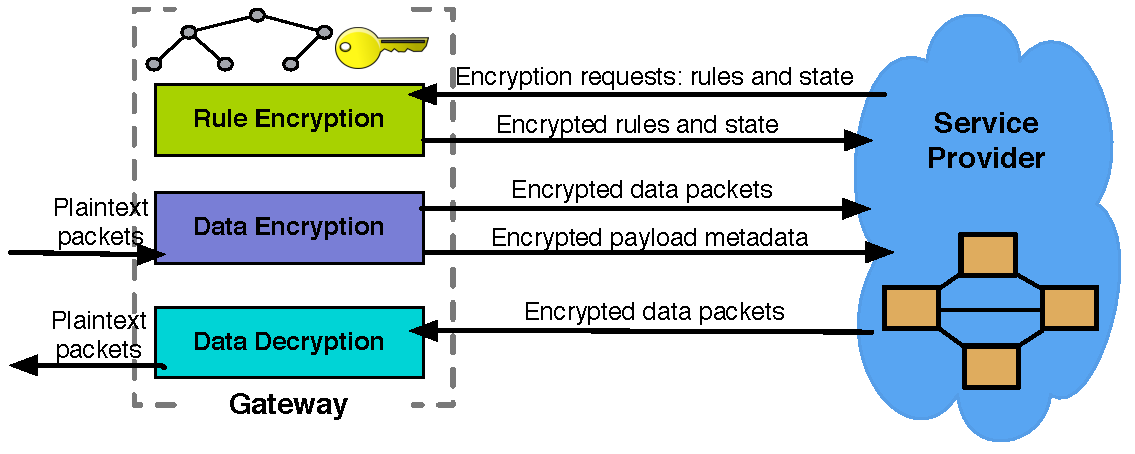
\includegraphics[width=3.25in]{fig/gateway2cloud}
  \caption[]{\label{fig:gatewaymeta} Communication between the cloud and gateway services: rule encryption, data encryption, and data decryption}
\end{figure}



\begin{figure}[t]
  \centering
  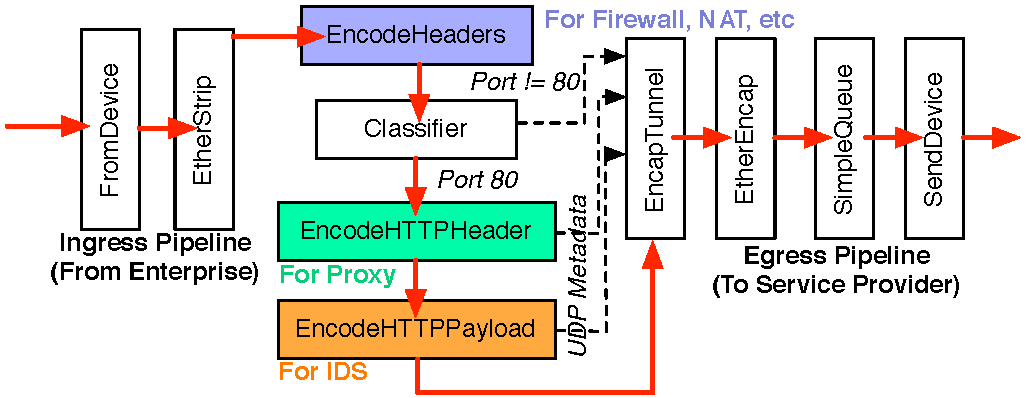
\includegraphics[width=3.25in]{fig/gatewaydiag}
  \caption[]{\label{fig:gateway} Data encryption (enterprise to cloud) click module.}
\end{figure}

The gateway serves two purposes. First, it redirects traffic to/from the cloud for middlebox processing. Second, it provides the cloud with encryptions of IDS/FW rulesets and updates to the RangeMatch tree.
Every gateway is configured statically to tunnel traffic to a fixed IP address at a single service provider point of presence.
A gateway can be logically thought of as three services: the rule encryption service, the pipeline from the enterprise to the cloud (Data encryption), and the pipeline from the cloud to the enterprise (Data decryption). 
All three services share access to the RangeMatch tree and the private key $k$.
Figure~\ref{fig:gatewaymeta} illustrates  these three services and the data they send to and from the cloud provider.

\noindent{\bf Rule Encryption.} The rule encryption component provides the cloud provider with encrypted rules/policies to use at the middlebox. 
There are two possible ways rules can be generated. First, an enterprise may choose to generate their own rules, in which case, they send encrypted versions of the rules directly to the cloud.
Rules can contain IP addresses, port numbers, and substrings of attack signatures; the first two must be encrypted with both keyword match and range match, the last needs only to be encrypted with keyword match.
Alternately, the enterprise may opt in to a `default' set of rules from the cloud provider, in which case the cloud provider sends the rules to the gateway which encrypts them and sends them back.
The rule encryption component also sends rule updates. Whenever an adjustment is made to the RangeMatch table, it sends an update to the cloud provider with the adjusted mappings/rules.
If the gateway ever changes its key, the encryption component must also signal to the cloud provider and re-encrypt all rules.
%\todo{too high level? Details about how updates work?}

\noindent{\bf Data Encryption.} In Figure~\ref{fig:gateway}, we show the DPDK-Click~\cite{click} packet processing pipeline that implements data encryption and transmits packets from the enterprise to the cloud.
Traffic that is returning from the Internet and traffic that is about to be sent to the Internet are both sent along this pipeline.
This figure assumes the enterprise is already using IPv6, if it is not, the pipeline would also include a `4to6' element.
In \S\ref{sec:overview}, we described how \sys encodes packet content using the AES, Keyword Match, and Range Match encryption algorithms. 
The encrypted values are placed either directly back in to a data packet, or transmitted over a {\it metadata channel}.
Below, we detail the three elements we implemented to encrypt the packet data:

\noindent {\it Encode Headers:} Encrypts the IP, TCP, and UDP headers, replacing all IP and Port numbers in the packet with values calculated using the {\it RangeMatch} encryption algorithm. Appends the AES-encrypted values to the IP options field of the data packet.
Required to support all middleboxes. 

\noindent {\it Encode HTTP Header.} Encrypts the HTTP header for {\it the first GET request only.} Does not modify the data packet itself, but instead places the keyword match encryptions of the values in a new packet sent over the metadata channel. 
The new packet marks (a) the encrypted 5-tuple flow ID for the packet, (b) that this is HTTP GET data for the proxy, and (c) the encrypted values. At the cloud, the proxy can read this metadata channel to obtain the encrypted URL for the GET request and check its cache for the encrypted data. This element is only needed if there is an HTTP proxy enabled at the cloud, otherwise it can be disabled at the gateway.

\noindent {\it Encode HTTP Payload.} Encrypts the entire HTTP payload (as described in \S\ref{sec:ids}), placing the keyword match values in a new packet in the metadata channel. Unlike the other two elements, this element keeps per-flow state, reconstructing the TCP stream in order to generate keyword match tokens for keywords which are divided across two subsequent packets.  The metadata channel packets contain (a) the encrypted 5-tuple for the packet, (b) that the packet contains keyword match data for the IDS, and (c) the encrypted values. At the cloud, the IDS can read this metadata channel to detect attacks; if there is a match it instructs the firewall to block the 5-tuple for the flow. This element is only needed if there is an IDS enabled at the cloud, otherwise it can be disabled at the gateway.


\noindent{\bf Data Decryption.} Packets returning from the cloud follow a much simpler packet processing pipeline than those being encrypted.
The packet payloads are decrypted using standard AES; the IP and port values from the options header are decrypted and then copied in to the packet header. The options header is removed.
If the enterprise is running IPv4, the traffic is sent back through the 4to6 converter to convert the packet back to IPv4.
The packet is then sent out to the Internet or the client at the enterprise.


\subsection{Middlebox implementations}
\label{sec:middleboxes}

\begin{figure}[t]
  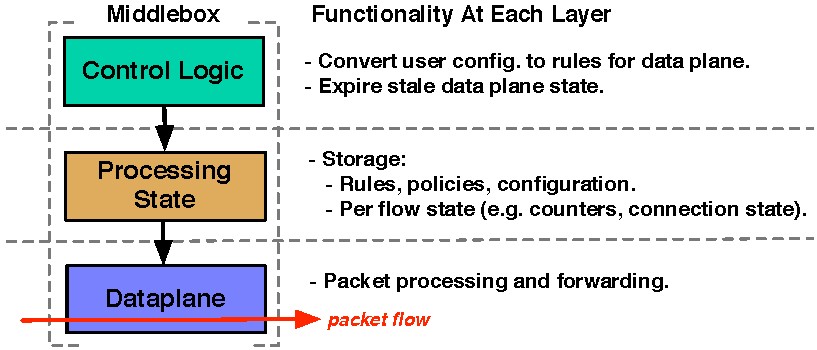
\includegraphics[width=3.25in]{fig/mbarch}
  \caption[]{\label{fig:mbarch} Typical middlebox software components. For most middleboxes, packet processing operations in the dataplane remain unmodified by \sys.}
\end{figure}

We implemented \sys for all middleboxes listed in Table~\ref{tab:apps-ops} using DPDK-Click~\cite{click}, with varying levels of modification to a baseline (unencrypted) design required to make them compatible with \sys. 
Figure~\ref{fig:mbarch} guides our discussion of these changes. %Most middlebox codebases can be divided in to three categories of functionality.
Although  middlebox software architectures are unlikely to be cleanly divided in to three independent components as shown, most classes and functions within a middlebox codebase can be labeled as one of these three categories.
These categories are: the dataplane (which performs packet processing), the middlebox state (which stores and updates rules and policies, as well as per-flow state like counters and connection state), and the control logic (which converts user configurations to rules and policies, and updates/refreshes state). 
Importantly, packet processing only occurs in dataplane functions, which are usually tightly engineered to process each packet in microseconds or faster.

We adapted all header-only middleboxes {\it without modifying steady-state dataplane functions}, and hence preserving the performance properties of the existing middleboxes.
We were able to do this because the encrypted values in the IPv6 header are stored in the normal IPv6 header formats, and because our encryption schemes preserve the exact match and range match semantics these devices use to operate correctly.
All we need to do to be compatible with normal dataplane behavior is to encrypt all values in the rules and configuration files using the the range match encryption algorithm.

We do need to change the control logic and add one `special case' check to the dataplane; this is to handle rule {\it updates}. 
The update code is triggered rarely -- when the gateway changes its key $k$, or when there is an update to the Range Match tree.
In this case the rules must be re-encrypted, and any per-session state (\eg{} the flow table in the NAT) must be re-encrypted as well.
When such an update is about to occur, the gateway first re-computes all rules {\it before} it begins to use the new encryption values on traffic. It signals to the cloud provider that it is about to perform a rule update. Then, all middleboxes transmit their rules / state tables to the gateway for re-encryption. 
Once all middleboxes have received their updated rules and state, the gateway `switches' to the new ruleset, sending a signal packet in the dataplane. When a middlebox receives this signal packet (the only change we make to the dataplane is to check for this signal packet) it switches out the ruleset to use the new values.~\footnote{\small There is a race condition for the flow state: consider a SYN packet which arrives just before the signal packet at a NAT. The NAT will encode the SYN packet in its state table using the old encryption scheme, and then immediately need to switch over to the new encryption scheme -- before it has the new mapping for the new flow. The middlebox will then immediately request a new encryption for the rule. Hence, a small number of packets may be misclassified during the transition.}
\todo{This is ugly as sin! Sigh! Can we do better?}  

Bytestream-aware middleboxes require changes in the dataplane as well as the control logic: \sys makes reading the payload directly impossible, and hence these middleboxes must be modified to operate over the metadata channel instead.
We re-implemented all such middleboxes from scratch.
However, these changes need not be a performance penalty: as we show in \S\ref{sec:eval}, we wrote an HTTP proxy from scratch to cache HTTP content; this proxy achieves comparable performance to existing, unencrypted proxies despite our encryption.
The primary difference between our proxy and a standard implementation is that the `table' storing file names/URIs and the file data is now over encrypted values; the content served is also opaque, encrypted data. 
In addition, the file names/URIs are read from the metadata channel, rather than the primary connection with the data packets. 
Otherwise, much of the more complicated aspects of the codebase (\eg{}, TCP session termination, storage and cache optimization, etc) can be implemented using out of the box libraries.

